\setstretch{1.0}
\chapter{From Source to Sensor: MEG Data Acquisition}

In this, the first theory chapter, an overview is provided on the processes which govern the generation and the detection of the magnetic fields which underpin MEG. Section \ref{sec_1_neuro} introduces the basic physiology of the neuron and explains the most likely origin of the MEG signal, along with types of neuromagnetic characteristics which are commonly observed. Section \ref{sec_SQUIDS} introduces the phenomenon of superconductivity, an electrical property of materials at ultra-low temperatures, and how we can exploit this to measure the tiny ($\sim10^{-15}$ T) changes in magnetic fields from neuronal ensembles. Section \ref{sec_1_inteference} discusses hardware and software techniques to reduce the effect of external sources of interference on MEG recordings, with particular focus on solutions used in the Nottingham laboratory.  Finally, Section \ref{sec_data_acq} discusses the protocols used to acquire all data used in this thesis. 

\doublespacing
\section{The neuronal origin of the MEG signal}\label{sec_1_neuro}

The human brain is the most complex biological structure in existance. Within its outermost layer, the cerebral cortex, exists on average $10^{10}$ cells. Between these cells exist around $10^{14}$ connections, which allow the passing of electrical and chemical signals \citep{Bear1996}. It is the time evolving magnetic fields associated with the passage of electrical currents flowing through neurons which an MEG system can detect. With current MEG hardware, the smallest current dipole which can be detected is $\sim$ 10 nAm \citep{Hamalainen1993}. As we show within this section, a current dipole of this strength requires coherence between an assembly of $\sim10^4$ current sources. However to understand what happens on this canonical scale, we need to first consider the processes within a single neuron.

\subsection{Electrophysiology of a single neuron}
A neuron can be broken down into five constituent parts as shown in Figure \ref{fig_1_b1}. 

\begin{itemize}
	\item \textbf{Soma:} Also known as the cell body, this is where the nucleus of cell resides.
	\item \textbf{Synapses:} Cell extrema which receive electrical signals and transmit chemicals called neurotransmitters for other neurons to detect. 
	\item \textbf{Dendrites:} Thread-like structures which are connected to neighbouring cells, these receive and pass on electrical impulses towards soma.
	\item \textbf{Axon:} A long slender structure which conducts electrical impulses away from the soma and onto other neurons. 
	\item \textbf{Axon Hillock:} The structure which initiates an action potential down the axon and towards neighbouring neurons when a threshold electric potential is exceeded.
\end{itemize} 

Neurons in the brain can be subcatagorised into two types based on their morphology. The first are known as stellate cells, which comprise the soma at the centre and an isotropic distribution of dentrides extruding radially. Due to their symmetry, it is believed that any electromagnetic field from dendritic currents of stellate cells cancel out and therefore do not contribute to the MEG signal. The second type are pyramidal cells, whose dendrites are oriented parallel to each other as depicted in Figure \ref{fig_1_b1}, which allow the magnetic fields of an assembly of pyramidal neurons to constructively superpose. It is believed therefore that pyramidal cells are the chief contributor to the extracranial fields observed in both MEG and EEG.

\begin{figure}[h!]
	\begin{center}
		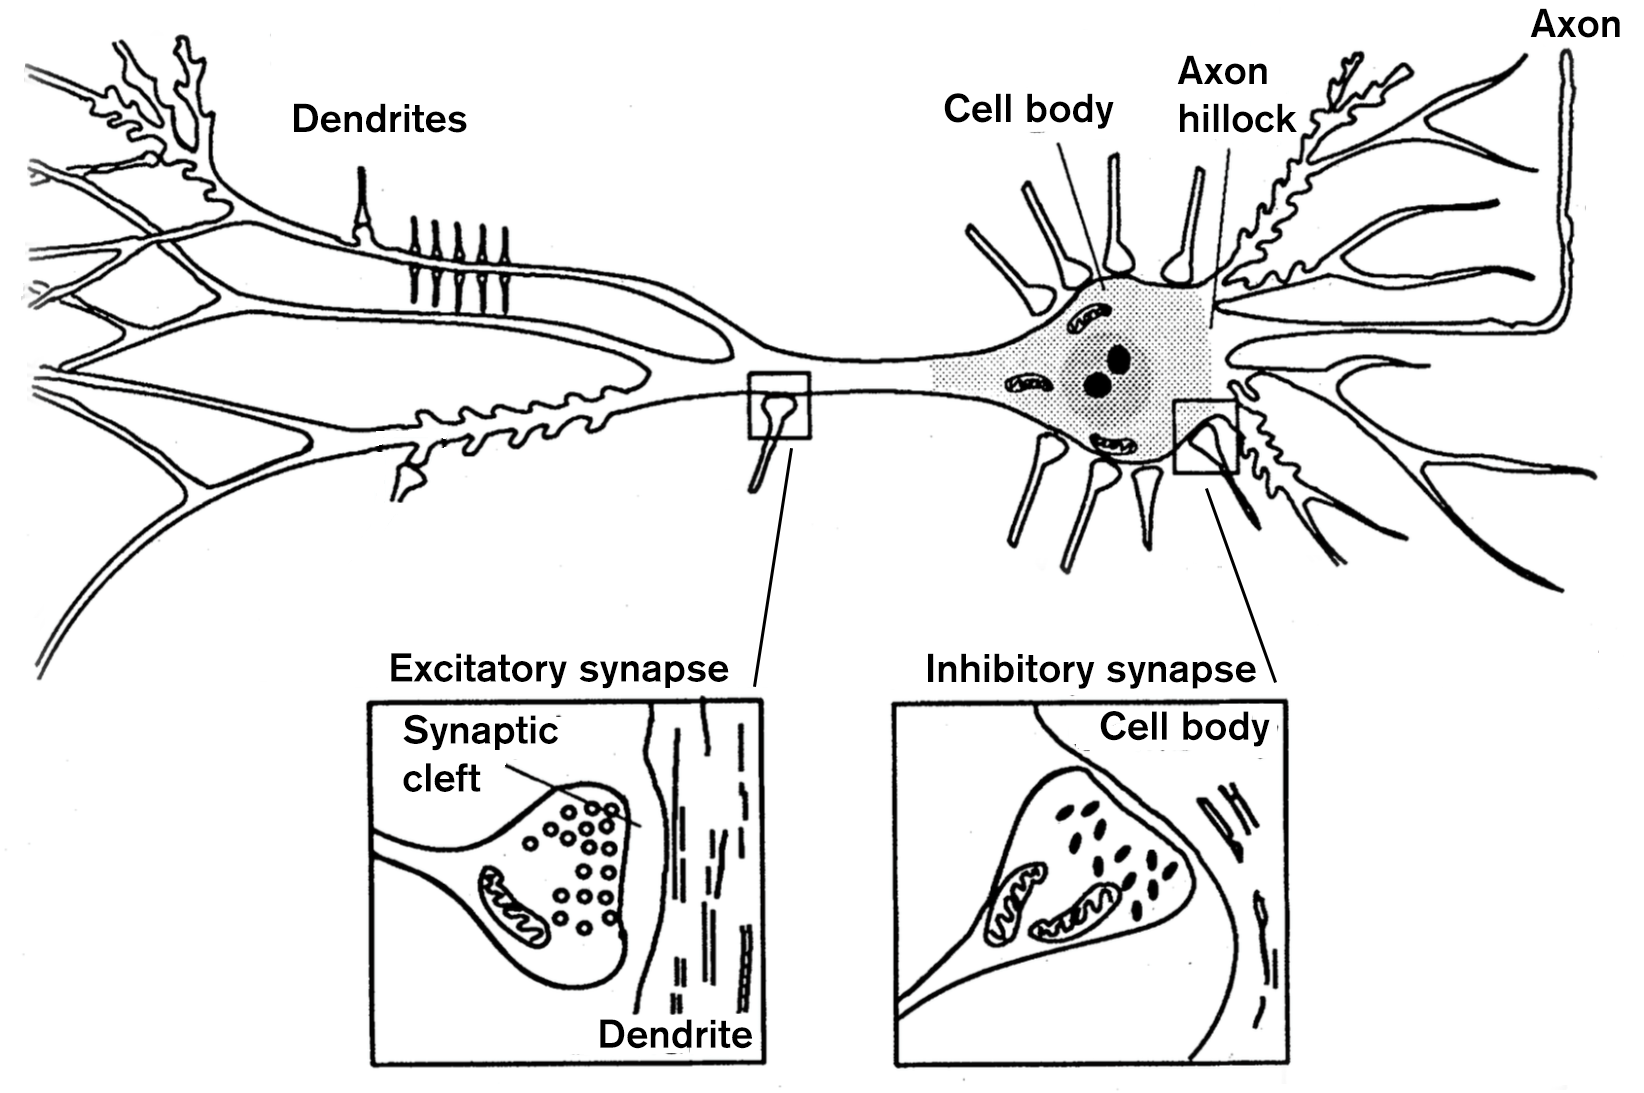
\includegraphics[width=\linewidth]{./images/chapter1/neuron.png}\caption{A schmatic representation of a pyramidal neuron. Figure adapted from \cite{Hamalainen1993}.}\label{fig_1_b1}
	\end{center}
\end{figure}

Information is propagated through neurons via a combination of electrical and chemical signalling processes. The membrane of the cell contains multiple ion channels, which when opened allow the passage of ions such as sodium (Na\textsuperscript{+}), potassium (K\textsuperscript{+}), and chlorine (Cl\textsuperscript{-}) in or out of the cell. These channels are either voltage-gated, which means they open when a potential threshold is met, or ligand-gated, when a specific neurotransmitter binds to it. Across the cell membrane, an electrical potential exists due to the build-up of the ions either side, and the opening of these channels allows for the modulation of this membrane potential. When the cell's ion concentration is at equilibrium across the membrane, it is said to be at its resting potential. The value of this is dictated by laws of thermodynamics; the concentration, \textit{C}, of each ion type will tend toward thermal equilibrium between the two sides of the membrane, which can be modelled by the Boltzmann equation

\begin{equation}
C \sim \text{exp}\Bigg(-\frac{|q|V}{k_BT}\Bigg),
\end{equation} where \textit{q} is the electron charge, \textit{V} is the potential difference across the membrane, $k_B$ is the Boltzmann constant and \textit{T} is the temperature. Rearranging this gives the Nernst equation, which allows us to calculate the potential difference across the membrane thus,

\begin{equation}
V = V_{\text{in}}-V_{\text{ext}}=\frac{k_B T}{|q|}\text{ln}\Bigg(\frac{C_{\text{in}}}{C_{\text{ext}}}\Bigg).
\end{equation} The resting potential across the membrane varies, but typically is around -70 mV \citep{Goldman1943}. 

\subsubsection{Action potentials}
If the potential at the axon hillock reaches a threshold (approximately -55 mV), it allows voltage-gated sodium and potassium ion channels to open. The concentrations of each ion either side of the membrane changes, with Na\textsuperscript{+} ions flowing in and K\textsuperscript{+} ions out of the neuron. At this critical potential the conductivity of sodium suddenly increases, causing a rapid influx of Na\textsuperscript{+} ions into the neuron, depolarising the membrane and raising the potential to 40 mV within 1-2 ms. This surge in potential difference is known as the \textit{action potential} and has the ability to raise the potential of adjacent membrane beyond their threshold, which triggers an action potential in a runaway process down the axon. After a spike in potential difference across a patch of membrane, the conductivity of sodium finally increases enough to cause an efflux of K\textsuperscript{+} ions, repolarising the membrane and lowering the potential back to the resting state almost as quick as was is raised. Action potentials, when propagating down the axon, can be thought of two opposing dipoles separated by a very small distance, meaning they can be modelled as a quadrupole. The magnetic field associated with quadrupoles falls with the cube of the distance, meaning the fields from action potential are very small at the surface of the scalp. However, a modelling study by \cite{Murakami2006} showed that the spiking associated from action potentials could be detected if 10000-50000 pyramidal cells spiked in unison. In practice, action potentials also have relatively short lifetimes (1-2 ms), meaning that the probability of synchrony on that scale is very low. It's for these reasons that action potentials are unlikely to be large contributors to the MEG signal, an observation which is supported by animal models on MEG signal origin \citep{Okada1997}.

\subsubsection{Post-synaptic potentials}
Connections between neurons are mediated by synaptic junctions. Here, communication is supported by a chemical rather than an electrical process. Once an action potential has propagated along the axon it reaches the synapse, where it stimulates the release of neurotransmitters. These neurotransmitters diffuse across a small (30-50 nm) gap known as the synaptic cleft (see Figure \ref{fig_1_b1}) to reach the receiving (or post-synaptic) neuron. Having crossed the cleft, neurotransmitters bind to the ligand-gated ion channels, opening them. Again the flow of ions through the membrane causes a change in the membrane potential, but this time depending on the junction type it either increases or decreases. If these ion channels allow the pumping of sodium and potassium ions, the potential increases, which are known as \textit{excitatory post-synaptic potentials} (EPSPs). Conversely if the channels which open allow for the pumping of chlorine, this serves to lower the potential in what are known as \textit{inhibitory post-synaptic potentials} (IPSPs). The likelihood of a neuron firing an action potential is dependent of the sum of the EPSPs and IPSPs reaching the critical threshold. An action potential will not occur should a single excitatory event occur, rather multiple events across the neuron in time will trigger the action potential to pass information to the next neuron. Likewise should an inhibitory event occur, the lowering of a potential reduces the chances of triggering. Post synaptic events create intracellular currents which flow across the synaptic junctions (due to the influx of ions) and along the dendrites toward the soma. The currents are dipolar and the resulting magnetic fields fall with distance squared and have a lifetime of 10 ms. The magnetic fields associated with PSPs are stronger at the head surface than those of action potentials and their longer lifetimes increase their probability of synchrony, which makes them a more likely source of the MEG signal. A consequence of this is that rather than measuring the output of neurons, MEG signals are instead dominated by the \textit{inputs} to cortical regions, so therefore are an indirect (and non-linear) measure of synaptic activity between neurons. 

\begin{figure}
	\begin{center}
		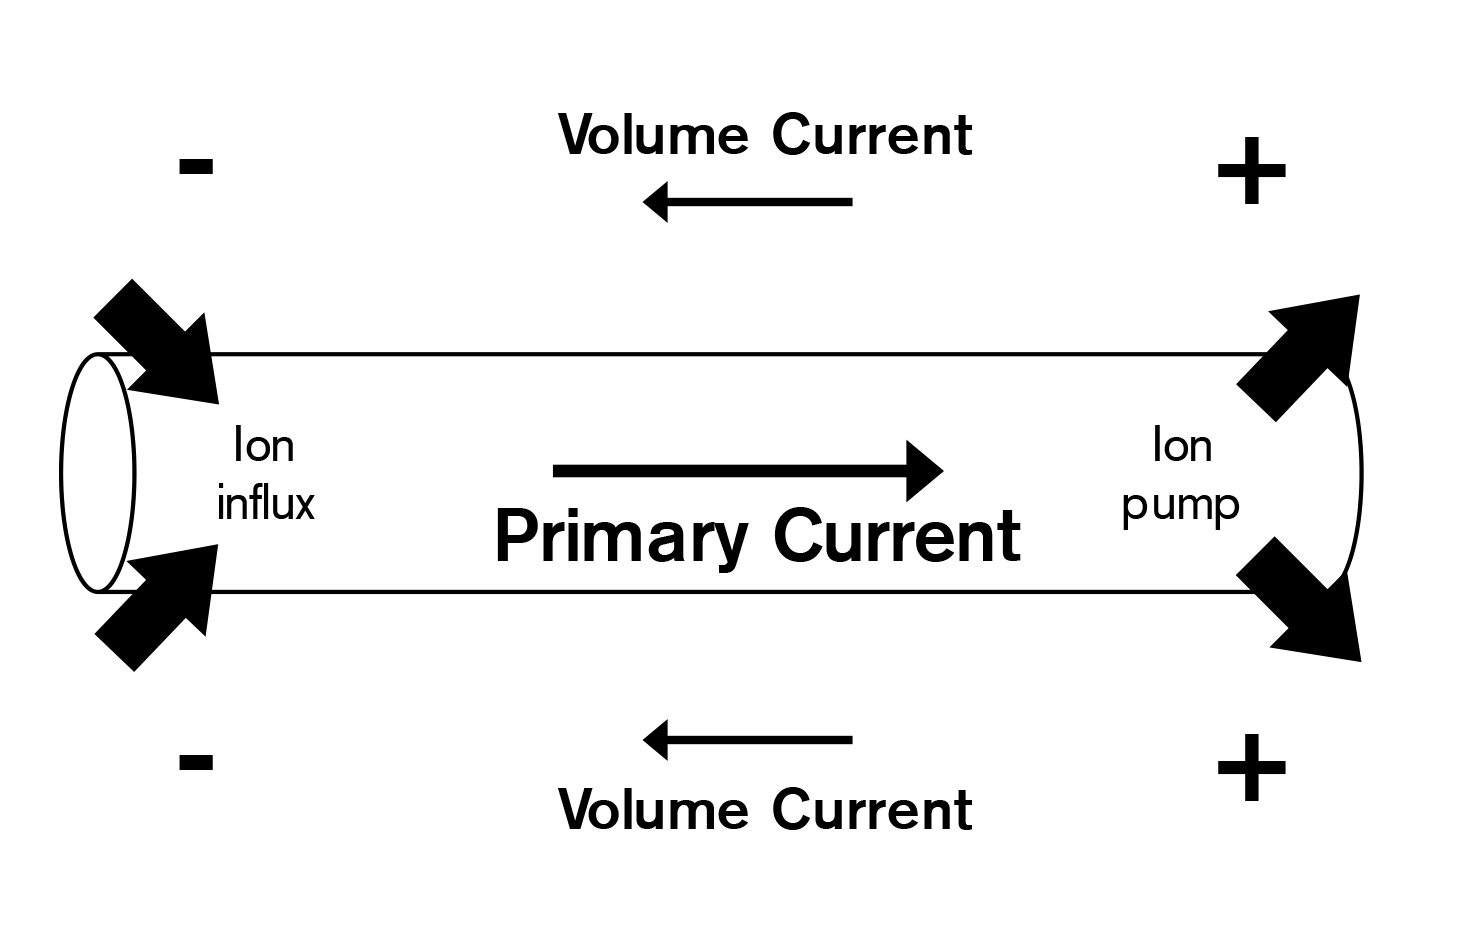
\includegraphics[width=0.8\linewidth]{./images/chapter1/dendrite.png}\caption{The post synaptic current along a dendrite. The primary current is caused by an influx of ions to the cell following the detection of neurotransmitters at a synaptic junction. The extracellular volume currents are the result of the electric field generated when ions are expelled. }\label{fig_1_b2}
	\end{center}
\end{figure}  

Following the passage of a post synaptic current, the resting potential of the cell must be restored (much like in the case of the axon). Here ion pumps expel ions back into extracellular space. The result of this process is the generation of an electric field between the ion expulsion point and the synaptic junction, which sets up an extracellular current in the opposite direction to the (primary) post synaptic current called the volume current (see Figure \ref{fig_1_b2}). However it will be shown in Chapter \ref{chapter_meg_source} that these volume currents have little effect on the measurable magnetic field.

The strength of a post-synaptic current dipole can be calculated through a series of experimental measures of neuronal properties. Typically the strength of a current source, \textit{i}, decays exponentially with distance from the influx of ions \textit{x} such that:

\begin{equation}
i(x) \propto \text{exp}\Bigg(-\frac{x}{\lambda}\Bigg)
\end{equation} where $\lambda$ is the characteristic length scale of the exponential decay, which is given by $\lambda=(\sigma_m\rho_f)^{0.5}$ where $\sigma_m$ is the conductance of the cell membrane and $\rho_f$ is the resistance per unit length of the intracellular fluid. For a cortical neuron, $\lambda$ is around 0.1-0.2 mm \citep{Scott1977}. Post synaptic currents can be modelled as current dipoles, which can be approximated by

\begin{equation}
Q_\text{PSP}=I\lambda.
\end{equation} The average post synaptic current can be estimated using the change of voltage $\Delta V$ thus

\begin{equation}
I = \frac{\Delta V}{\lambda\rho_f}.
\end{equation} If we use \textit{d} to represent the diameter of the dendrite and $\sigma_f$ the conductivity of the intracellular fluid, then we find that.

\begin{equation}
Q_\text{PSP}=\frac{\pi d^2\sigma_f \Delta V}{4}.
\end{equation} Inserting typical values ($d=1$ μm, $\sigma_f=1$ Ω\textsuperscript{-1}m\textsuperscript{-1} and $\Delta V=25$ mv) we find that for a single post synaptic potential, $Q\approx20$ fAm. To summarise the current section, the evidence suggests that the neuronal origin of the MEG signal is from the synchronisation of at least $10^4$ dendritic currents arising from pyramidal cells. 

\subsection{Measurable neuromagnetic phenomena}
The neuromagnetic fields which an MEG system is capable of detecting have rich temporal and spectral properties associated with them. Depending how the recordings signals are analysed (selection of filtering bands, or how data are averaged for example) has profound effects on the results. Below are two such types of neuromagnetic phenomena commonly assessed with MEG.

\subsubsection{Evoked responses}
Many studies involving MEG have typically focussed on evoked responses. These responses are time and phase locked to either the onset or offset of an external stimulus, which results in a characteristic spike in the measured magnetic field strength. Studies into evoked responses typically have involved their detection in the visual \citep{Ahlfors1992}, somatosensory \citep{Hari1990} or auditory cortices \citep{Makela1990} and experiments typically involve a stimulus being presented to a subject over the course of multiple trials. Here, the time and phase locked nature of the evoked response means that, after averaging the MEG data across trials, random (non phase locked) fluctuations are attenuated, revealing the prominent evoked signal. The enhancement in signal-to-noise ratio (SNR) from trial averaging is proportional to the number or trials recorded, \textit{n} such that, assuming Gaussian noise,

\begin{equation}
\epsilon_\text{SNR} = \sqrt{n}.
\end{equation} In addition to trial averaging we can drive the brain to produce \textit{steady state} evoked responses \citep{Regan1977} by driving a stimulus on and off at high frequency. This results in the evoked responses resonate at a characteristic frequency typically associated with the stimulus frequency. The role of evoked responses in functional connectivity has not been particularly well characterised, but there are some studies which have shown evoked responses between regions being 'connected'. For example invasive recordings have shown synchronised cortico-cortical evoked potentials between Broca's and Wernicke's areas when either area was stimulated \citep{Matsumoto2004}. Studies in EEG have shown that the strength of the evoked response in the auditory cortices in an oddball task is proportional to the strength of the connectivity between the regions \citep{Kuhnis2014}, however it hasn't been determined which process drives which.  

\subsubsection{Spontaneous oscillations} 
The other common phenomenon which can be observed with MEG are spontaneous oscillations. These were first discovered using EEG by Hans Berger \citeyearpar{Berger1929}. What he found was that when measuring electrical potential differences across the scalp surface, characteristic oscillations of between 8-13 Hz existed in the occipital lobe of the brain. Further the amplitude of this wave could be attenuated by visual stimulation. Since then much work has been done to characterise oscillations in the brain and several frequency bands have been categorised. These range from low frequencies (Delta, <4 Hz; Theta, 4-8 Hz) to higher (Alpha, 8-13 Hz; Beta, 13-30 Hz; Gamma >30 Hz) and even ultra-high (Sigma > 400 Hz; Kappa > 800 Hz; \citealp{Fedele2015}). High frequency oscillations may also be referred to as ripples (80-250 Hz) or fast ripples (250–1000 Hz) in the literature \citep{Buzsaki1992,Bragin2002,Worrell2008}, and some of the lower frequency bands may also be split further (e.g Alpha is often split into two narrower bands of 8-10 Hz and 10-13 Hz respectively as these can behave distinctly to each other \citep{Bosboom2008,vanderMeer2013,Hillebrand2016}) Much like the Berger study, it has been shown that the amplitude of the oscillations can be modulated in the presence of a task \citep{Pfurtscheller1999,vanBurik1999,Singh2002}. Unlike evoked responses, whilst time locked, event related changes in oscillations are not phase locked, so simple trial averaging cannot be used because their non phase locked nature causes spontaneous oscillations to average to zero.

\begin{figure}
	\includegraphics[width=\linewidth]{./images/chapter1/Figure_osc.png}\caption{The relation of neuronal oscillations and functional connections. A) A function of cell excitability over time; at peak excitability are the spiking events associated with action potentials. B) A model of communications between neurons based on the model neuronal coherence \citep{Fries2005}, which suggests neurons which are in phase with each other are likely to be functionally connected.}\label{figure_1_osc}
\end{figure}

A model for relating neuronal oscillations to long range communication in the brain was proposed by \cite{Fries2005}, which describes communication through neuronal coherence. The schematic of this model can be found in Figure \ref{figure_1_osc}. This model argues that communication is dependent on the transmitter and receiver needing to coherently oscillate with each other to optimally send information. The excitability of a neuron is dependent of the phase on the neuronal oscillation, so at peak excitability spiking can occur (Figure \ref{figure_1_osc}A). Likewise, at peak excitability a neuron is best positioned to receive electrochemical signals, so should two oscillations be sufficiently in phase with each other (such as the red and green signals in Figure \ref{figure_1_osc}B) they are more likely to be functionally connected to each other. An attractive feature of neuronal oscillations is that they are present even in the absence of a task, which has made them popular for analysing functional connectivity in both resting state and task-based paradigms. It is these neuronal oscillations which are the main focus of functional connectivity studies using MEG, as their spatial signatures have been shown by many studies to resemble networks fMRI \citep{dePasquale2010,Brookes2011,Brookes2011a,Luckhoo2012,Hipp2012,Marzetti2013,Baker2014,Florin2015}. In addition the relative ease of data acquisition compared to a task (especially in patients who may find it difficult or unnerving to execute) and the ability to combine data from multiple studies with little difficult make it an attractive paradigm for many. However in this case, ease of data acquisition trades off with difficulty of analysis, as mentioned to in Chapter \ref{chap_intro}, the lack of time locked events in the data makes it difficult to assess what is a genuine change in connectivity and what is a spurious phenomenon \citep{Hindriks2016}. In additionally it has been shown in the resting state, the patterns of inter-subject differences may be distinct to the differences seen in a single subject who has undergone multiple acquisitions \citep{Laumann2015}, which may make stratification via functional connectivity metrics harder to achieve in the resting state. 

\section{MEG signal detection}\label{sec_SQUIDS}
The task of detecting neuromagnetic fields from the brain is non-trivial, as the fields in question are of the order of 100 fT. In the original 1968 paper by Cohen and colleagues, the magnetic fields from the brain were detected with a large pick up coil made of $\sim$10\textsuperscript{6} turns \citep{Cohen1968}. This was quickly superseded by Superconducting Quantum Interference Devices (SQUIDs) to measure neuromagnetic fields \citep{Cohen1972}, which at the time of writing this thesis are the only method used in commercially available MEG systems\footnote{There is some exciting work being done investigating the feasibility of optically pumped magnetometers (OPMs) as a successor to SQUIDs. In short, these have the attractive quality of being cryogenic free which may remove many hardware constraints which come with having to keep your magnetometers below 4.4 K.}. In this section, the fundamental concepts behind how SQUIDs operate are discussed. There will be particular emphasis on methods used by the CTF MEG 275-channel system located at the Sir Peter Mansfield Imaging Centre, which is where all experimental data were recorded for this thesis.  

\subsection{Superconductivity}
Discovered in 1911 by Heike Kamerlingh Onnes, superconductivity is the phenomenon that at low temperatures (on the order of a few Kelvin), the electrical resistance of some materials falls to 0 $\Omega$, allowing them to form a perfect conductor \citep{Onnes1911}. It had been postulated that resistance gradually fell with temperature, but what Onnes showed was that at a critical transition temperature $T_c$, the resistance of some metals abruptly drops. Further research has shown that superconducting materials exist in one of two categories. All superconducting material exhibits what is known as the Meissner effect, where due to screening currents on the surface of the material, all magnetic fields within a superconductor are expelled \citep{Meissner1933}. However it was shown that in type-I superconductors, which typically are elemental metals (save for niobium, vanadium and technitium), given a strong enough field, $\mathbf{B}_C$, superconductivity could be destroyed. Type-II superconductors, which are primarily alloys have two critical magnetic fields, $\mathbf{B}_{C1}$ and $\mathbf{B}_{C2}$, where $\mathbf{B}_{C1} << \mathbf{B}_{C2}$. When a field stronger or equal to $\mathbf{B}_{C1}$ is applied to a type-II superconductor, magnetic flux is allowed to permeate the materal, and the density of the flux rises with field strength until at $\mathbf{B}_{C2}$ all superconductivity is destroyed \citep{Rjabinin1935}. The main advantage with type-II superconductors is that they can maintain superconductivity in the presence of a much stronger magnetic field, for this reason SQUIDs are made from such materials.      

In 1957, a microscopic theory was proposed by Bardeen, Cooper and Schrieffer, to explain the peculiar effects seen in superconductors, and today this is known as BCS theory \citep{Bardeen1957}. BCS theory states that when an electron passes through a lattice of phonons, it causes the lattice to distort towards it (analogous to the wake of a ship), creating a build up of positive charge in the vicinity. If a second electron is sufficiently near (under 100 nm), then it is attracted to this area of positive charge. These electrons become bound in a structure known as a Cooper pair. This seems somewhat counter-intuitive, as we would expect the Coulomb interaction to repel the electrons from each other. However, this is partly screened out by the other electrons in the vicinity and the attraction to the positive charge from lattice distortion being dominant. The thermal energy required to break the bond between pairs is on the order of $10^{-3}$ eV, so it is only at low temperatures that these pairs survive. Cooper pairs act like a Boson, so many are allowed to exist in the same quantum mechanical state. BCS theory showed that superconductivity is a cooperative phenomenon, such that the binding energy between cooper pairs increases as more pairs come to exist in the same state. A consequence is that the motion of the centre of mass for all these pairs must be equivalent, i.e. all pairs must be travelling in the same direction with the same momentum. It is this that mediates a supercurrent.

The wavefunctions of individual Cooper pairs constructively interfere to form a canonical wavefunction of the entire system, known as an \textit{order parameter} which allows us to observe quantum effects at the macroscale. If we ignore the relative motion of the individual electrons of the Cooper pair, we see that our order parameter is dependent only on the centre of mass between two electrons, \textbf{r} and their momentum $\hbar\mathbf{q}$:

\begin{equation}
\psi(\mathbf{r})=\psi_0\text{e}^{i\mathbf{q}.\mathbf{r}} \label{eqn_1_3}
\end{equation} where $\psi_0$ is the wavefunction of the Cooper pair ground state. What this equation tells us is that the wavefunction propagates as an oscillator, with maximal likelihood of being found at the centre of mass \textbf{r}.

\subsection{Flux quantization}
Let's use Equation \ref{eqn_1_3} to investigate what happens within a superconducting medium. The current density of the wavefunction can be defined as \citep{London1948,Hook1991}

\begin{equation}
\mathbf{j}(\mathbf{r}) = \frac{i\hbar e}{2m}(\psi^*\mathbf{\nabla}\psi-\psi\mathbf{\nabla}\psi^*)-\frac{2e^2}{m}\psi^*\psi\mathbf{A} \label{eqn_1_4}
\end{equation} where $e$ is the fundamental electron charge, $m$ is the electron mass, $\hbar$ is the  reduced Planck constant and \textbf{A} is the magnetic vector potential. Generalising \ref{eqn_1_3} so
 $\psi(\mathbf{r})=|\psi_0|\text{e}^{i\theta(\mathbf{r})}$, where $\theta(\mathbf{r})=\mathbf{q}.\mathbf{r}$ and inserting it into Equation \ref{eqn_1_4} gives %\footnote{Not only Equation \ref{eqn_1_5}, but a spontaneous nosebleed to whoever tries to derive this!}

\begin{equation}
	\begin{aligned}
		\mathbf{j}(\mathbf{r}) &=  \frac{i\hbar e}{2m}\Bigg(\psi_0\text{e}^{-i\theta}\Big(\text{e}^{i\theta}\mathbf{\nabla}\psi_0+i\psi_0\text{e}^{i\theta}\mathbf{\nabla}\theta\Big)-\psi_0\text{e}^{i\theta}\Big(\text{e}^{-i\theta}\mathbf{\nabla}\psi_0-i\psi_0\text{e}^{-i\theta}\mathbf{\nabla}\theta\Big)\Bigg)
	 -\frac{2e^2}{m}|\psi(\mathbf{r})|^2\mathbf{A} \\
	 &= \frac{i\hbar e}{2m}\Big(2i|\psi(\mathbf{r})|^2\mathbf{\nabla}\theta\Big)-\frac{2e^2}{m}|\psi(\mathbf{r})|^2\mathbf{A} \\
		&= -(e/m)|\psi(\mathbf{r})|^2(\hbar\mathbf{\nabla}\theta+2e\mathbf{A})\label{eqn_1_5}
	\end{aligned}
\end{equation} Now, far from the surface of a superconductor, \textbf{j}=0, so Equation \ref{eqn_1_5} then becomes 

\begin{equation}
\hbar\mathbf{\nabla}\theta = -2e\mathbf{A}. \label{eqn_1_6}
\end{equation} If we intergrate this equation around a closed curve, \textit{C} within the superconductor,

\begin{equation}
	\begin{aligned}
		\hbar \oint_C \mathbf{\nabla}\theta.\text{d}\mathbf{l} &= \hbar\Delta\theta \\
		&= -2e\oint_C \mathbf{A}.\text{d}\mathbf{l}.
	\end{aligned} 
\end{equation} Since the order parameter is a wavefunction, it must follow that the properties and the boundary conditions must also follow the same laws. Therefore, the order parameter must be single valued and the phase change around the closed loop, $\Delta\theta$ must be $2\pi n$, where $n \in \mathbb{Z}$. To solve the integral $\oint_C \mathbf{A}.\text{d}\mathbf{l}$, we recall Stokes theorem, and transform the line integral into a surface integral 

\begin{equation}
-2e\oint_C \mathbf{A}.\text{d}\mathbf{l} = -2e \iint_S \mathbf{\nabla} \times \mathbf{A}.\text{d}\mathbf{S},
\end{equation} where the surface \textit{S} is bound by the closed loop \textit{C}. Given that $\mathbf{\nabla}\times\mathbf{A}=\mathbf{B}$, it therefore follows that 

\begin{equation}
\begin{aligned}
2\pi n \hbar &=-2e\iint_S \mathbf{B}.\text{d}\mathbf{S} \\
&= -2e\Phi.
\end{aligned} \label{eqn_1_9}
\end{equation} What the result in Equation \ref{eqn_1_9} shows us is that the amount of flux through a closed loop of arbitrary geometry is quantised. The quantisation is such that $\Phi=n\Phi_0$, where $\Phi_0 = h/2e$ is the flux quantum and has a value of $2.07 \times 10^{-15}$ Wb.
\subsection{Josephson junctions}
In 1962 Brian David Josephson postulated that if two layers of supercondutive material were separated by a weakly coupled insulator, Cooper pairs should still be able to tunnel through the gap when $T < T_c$, even in the absence of an applied voltage \citep{Josephson1962}. This is analogous to how an electron can tunnel though a potential barrier, but at a macroscopic level.  

Consider two superconductors with order parameters $\psi_1 = |\psi_1|\text{e}^{i\theta_1}$ and $\psi_2 = |\psi_2|\text{e}^{i\theta_2}$ respectively. If the two superconductors are sufficiently far apart from each other, but at the same temperature, $|\psi_1| = |\psi_2|$, but due to the lack of interaction we generally find that $\theta_1 \neq \theta_2$. If the two are brought into contact with each other, the two order parameters must equate and so the phases of each order parameter must equalise. Now, consider the two superconductors are separated by an 'insulating' layer (such as Al\textsubscript{3}O\textsubscript{2} or MgO\textsubscript{2}) of thickness \textit{d} (as shown in Figure \ref{fig_1_s1}). Here, the order parameters are weakly coupled (i.e the energy scale of the coupling is much lower than of the order parameter itself), and the lowest energy state is still one where $\theta_1 = \theta_2$. However, it is possible to generate a difference in phase across the oxide layer by either forcing a current through the coupling, or applying a potential difference across it. Two order parameters weakly coupled in a setup like this are said to form a \textit{Josephson junction}. 

Below $T_c$, it is possible for Cooper pairs to tunnel through the oxide barrier, even in the absence of a voltage across it. The tunnelling is a result of the order parameters for each superconductor extending into the gap. Figure \ref{fig_1_s1} shows this and the exponential decay of the order parameter as it tunnels further into the oxide layer. Within the gap itself, the two order parameters superpose; assuming that each of the order parameters make very little contribution to the other post-tunnelling, the order parameter within the gap is 

\begin{figure}[t!]
	\begin{center}
		\includegraphics[width=\linewidth]{./images/chapter1/figure_s1.png}\caption{A) A schematic Josephson junction, which consists of two layers of superconducting material surrounding an "insulating" oxide layer. Order parameters either side of oxide layer can tunnel through at sufficiently low temperatures, meaning there is a weak interaction between $\Psi_1$ and $\Psi_2$. B) A simplified diagram of a SQUID, containing two Josephson junctions connected in parallel. Current through the ring is dependent on the flux $\Phi$ cutting the ring. The blue curves represent the line integrals used in Equation \ref{eqn_1_13}.}\label{fig_1_s1}
	\end{center}
\end{figure}

\begin{equation}
\psi=\Bigg(\frac{n_s}{2}\Bigg)^{\frac{1}{2}}\Big(\text{e}^{i\theta_1-K(x+d/2)}+\text{e}^{i\theta_2+K(x-d/2)}\Big). \label{eqn_1_10}
\end{equation} The barrier extends from $-\frac{d}{2} \leq x \leq \frac{d}{2}$, $n_s$ is the number of charged particles per unit volume (the factor of 0.5 comes from there being 2 electrons for every Cooper pair) and $K^{-1}$ is the characteristic decay length of the barrier. To calculate the current density, we use Equation \ref{eqn_1_4}, with the vector potential, $\mathbf{A}=0$ and the order parameter in Equation \ref{eqn_1_10} to find

\begin{equation}
\begin{aligned}
 j &= \frac{ie\hbar n_s}{2m}K\text{e}^{-Kd}\Big(-\text{e}^{i(\theta_1-\theta_2)}+\text{e}^{i(\theta_2-\theta_1)}\Big) \\
 &= j_0\text{sin}(\delta) \label{eqn_1_11}
\end{aligned}
\end{equation} where $j_0 = \frac{e\hbar n_s}{m}K\text{e}^{-Kd}$ is the critical current density and $\delta = \theta_1 - \theta_2$. If a current is caused to flow through the junction, the phase difference adjusts accordingly so that Equation \ref{eqn_1_11}, known as Josephson equation, is satisfied. The existance of cooper pair flow across the junction is known as the \textit{DC Josephson effect.}


\subsection{Quantum interference}
Consider two Josephson junctions in parallel with each other, connected by super conducting material to form a loop as shown in Figure \ref{fig_1_s1}. The combined tunnelling current across both junctions is
\begin{equation}
\begin{aligned}
I &= I_A + I_B \\
&= Aj_o\big[\text{sin}(\delta_A)+\text{sin}(\delta_B)\big] \\
&=2Aj_c\text{cos}\Bigg(\frac{\delta_A-\delta_B}{2}\Bigg)\text{sin}\Bigg(\frac{\delta_A+\delta_B}{2}\Bigg)
\end{aligned} \label{eqn_1_12}
\end{equation} where \textit{A} is the surface area of each junction and the phase differences across each junction are denoted as $\delta_A$ and $\delta_B$. We now use a similar technique to that used to prove flux quantization to show that $\delta_A-\delta_B$ is determined by the magnetic flux through the loop. Because the current density is a vanishing term within the bulk of the superconducting material, Equation \ref{eqn_1_6} remains valid. If we integrate along the paths shown as the blue lines in Figure \ref{fig_1_s1}, we find

\begin{equation}
\begin{aligned}
\theta_{\text{a1}} - \theta_{\text{b1}} &= \frac{2e}{\hbar}\int_{C1} \mathbf{A}.\text{d}\mathbf{l} \\ \theta_{\text{a2}} - \theta_{\text{b2}} &= \frac{2e}{\hbar}\int_{C2} \mathbf{A}.\text{d}\mathbf{l}
\end{aligned} \label{eqn_1_13}
\end{equation} where $\theta_\text{a1}$, $\theta_\text{b1}$, $\theta_\text{a2}$ and $\theta_\text{b2}$ are the phases at the ends of the curves $C_1$ and $C_2$ close to the junctions indicated by the subscripts. Adding these equations we find

\begin{equation}
\begin{aligned}
\delta_A - \delta_B &= \frac{2e}{\hbar}\oint_C\mathbf{A}.\text{d}\mathbf{l} \\
&\approx  \frac{2e\Phi}{\hbar}. \label{eqn_1_14}
\end{aligned}
\end{equation} Note the approximation sign, as we have neglected to include the contributions from the junctions themselves, but these extra terms are negligible. Inserting Equation \ref{eqn_1_14} into \ref{eqn_1_12} gives

\begin{equation}
I=2Aj_c\text{cos}\Bigg(\frac{e}{\hbar}\Phi\Bigg)\text{sin}\Bigg(\frac{\delta_A+\delta_B}{2}\Bigg)
\end{equation} which resembles the Equation \ref{eqn_1_11}, describing the current density for a single junction. In the case of a double junction rather than $\theta_1 - \theta_2$ varying to allow a current to pass through, it is instead $\frac{\delta_A+\delta_B}{2}$. The maximum supercurrent which the junctions can now carry is

\begin{equation}
I_{\text{max}} = 2Aj_0\Bigg|\text{cos}\Bigg(\frac{e}{\hbar}\Phi\Bigg)\Bigg| \label{eqn_1_16}
\end{equation} which varies periodically with the flux crossing through the ring, with the period being the flux quantum, $\Phi_0$. Because the flux quantum is such a small quantity, the device described in Figure \ref{fig_1_s1}, if it had a junction surface area of 1 cm\textsuperscript{2}, would run from minimum to maximum current in only $10^{-11}$ T. This is the basic premise for a superconducting quantum interference device (SQUID) and is the reason it can be used as a sensitive device for measurement of small magnetic fields. 

\subsection{DC SQUID operation}

As established above, the tunnelling of Cooper pairs allows small currents to flow through the SQUID. However should the current exceed a critical value, $I_c$, the junctions start to have resistive properties. This in turn induces a drop in potential difference across the device. If we apply a bias current through the SQUID which is larger than $I_c$ then the change in magnetic fields will no longer induce a change in current (as described in Equation \ref{eqn_1_16}), but rather a change in the potential difference across the SQUID. This voltage modulation is what is used in the detection of small neuromagnetic fields by a SQUID in a MEG system. 

Figure \ref{fig_1_s2}A shows a digram of the circuitry of a DC SQUID, which shows how the SQUID can be connected to a flux transformer which shares a mutual inductance \textit{M}. This allows the SQUID itself to be located distal to the head surface which allows it to be shielded from interference. When the bias current exceeds the critical current, the potential difference across the SQUID follows the periodic behaviour shown in Figure \ref{fig_1_s2}B when modulated by flux .The SQUID operates on the steepest part of the response curve, where the transfer function $V_\Phi = \frac{\text{d}V}{\text{d}\Phi}$ is at its steepest. This is called the lock point and a feedback loop ensures it stays at that point. In short this is how a DC SQUID operates:

\begin{enumerate}
	\item Time varying neuromagnetic fields cause current variation in the pickup coil, $L_P$. This in turn causes current flow in the signal coil $L_S$.
	\item The signal coil is coupled to the SQUID ring via a mutual inductance, \textit{M}. The current in the signal coil therefore alters the flux cutting the ring.
	\item The ring responds with additional currents to compensate for the field. However as the SQUID has been saturated with the bias current, the result is a fall in the potential difference across the ring.
	\item The drop in potential is detected by the SQUID electronics, which responds by passing feedback current through the ring to counterbalance the induced current.
	\item The output of the feedback is measured as a voltage produced across a load resistor in the feedback circuit. This acts as the magnetometer output. 
\end{enumerate} 

\begin{figure}
	\begin{center}
		\includegraphics[width=0.75\linewidth]{./images/chapter1/figure_s2.png}\caption{A) The schematic diagram of a DC squid. B) The transfer function which shows the flux to voltage response of the DC SQUID.}\label{fig_1_s2}
	\end{center}
\end{figure}

\subsection{SQUID dynamic range \& resolution}
Because of the periodicity of the transfer function, it appears initially difficult to measure changes in the magnetic field larger than $\pm\frac{1}{4}\Phi_0$ from a lock point before you have multiple solutions to a single potential difference reading. This can be circumvented with the addition of a flux modulation circuit \citep{Forgacs1967}. The flux modulator adds a rapid square wave modulation of flux into the SQUID as shown in Figure \ref{fig_1_s3}A, (which for the CTF MEG system in Nottingham, ranges from $\pm\frac{1}{4}\Phi_0$ at a frequency $f_{mod} = 192$ kHz). By inspecting how the high frequency modulation manifests itself in the SQUID readout, we can determine the current phase of the transfer function, allowing us a true dynamic range of $\pm\Phi_0$. For the Nottingham CTF system, $\Phi_0$ equates to a field change of approximately 330 pT for a head sensor. In addition, the dynamic resolution of the SQUID is limited only by how precisely one can measure the voltage. In our case the CTF system uses a 20-bit Analog to Digital Converter (ADC) to digitise the signal, allowing for a dynamic resolution of 0.3 fT per least significant bit. 

However over time the field will drift further than $\pm\Phi_0$ due to multiple environmental factors (see Section \ref{sec_1_inteference} for examples), and so this needs to be accounted for. We can take advantage of the periodicity of the transfer function to artificially extend the dynamic range of the SQUID further. Whenever an integer multiple of $\Phi_0$ has been exceeded, the loop lock disengages and the SQUID is reset back to its lock point. A counter then adds plus or minus 1 to the current value to indicate a reset has occurred. A graphical description is shown in Figure \ref{fig_1_s3}B. Here the digitised signal and the reset count are merged to reconstruct a signal which modulates over multiple $\Phi_0$. The number of periods from the original lock point is currently limited by how far a computer can count to. On a 32-bit system, if 20 bits are reserved for the digitised signal, there are 12 remaining bits for the counter. This results in a signal range of $\pm 2048 \Phi_0$, or $\pm680$ nT, which is potentially far below the physical operating range of the SQUID itself\footnote{CTF scanners are due an electronic and software upgrade to handle 64 bit data in the immediate future, so in theory this signal range can be extended much further. Assuming that the signal digitisation is performed with 24-bit ADC (which are readily available), this leaves 40 bits for the counter. The result of this would be a theoretical resolution of 20 aT, and a signal range of $\pm 360$ T! Whilst these limits are \textit{probably} unattainable, it does mean that we could operate the SQUID across its true physical range.}. Using this reset system requires fewer SQUID tunings of the MEG system (a system with this feature can go months instead of days without retuning); however, the drawback is a SQUID reset artefact is considerably larger than the signal arising from neuromagnetic field, so for good data large changes in magnetic field should be best avoided.    

\begin{figure}
	\begin{center}
		\includegraphics[width=\linewidth]{./images/chapter1/figure_s3.png}\caption{Methods used to extend the dynamic range of a DC SQUID. A) The process of flux modulation, where a high frequency flux oscillation is applied to the SQUID. The intensity and phase of the corresponding high frequency potential difference measurement determines where on the transfer function a SQUID currently resides. B) A schematic showing how MEG electronics can deal with a signal which deviates more than 1 $\Phi_0$ by performing SQUID resets. Panels A and B adapted from \cite{Hamalainen1993} and \cite{Vrba1999} respectively.}\label{fig_1_s3}
	\end{center}
\end{figure}

\clearpage

\section{Interference reduction}\label{sec_1_inteference}
So far we have established that the neuromagnetic fields measured by MEG are on the order of 100 fT and shown that SQUIDs are sensitive and resolute enough to detect changes in magnetic fields at this scale. However these fields are approximately $10^{8}$ times smaller than the Earth's magnetic field and  orders of magnitude smaller than magnetic sources from lab instrumentation, passing vehicles and even other biological processes. Examples of such sources and their field strengths are shown in Figure \ref{fig_1_n0}. This makes the measurement of neuromagnetic fields problematic, and so both hardware and software oriented solutions need to be implemented in MEG.

\begin{figure}
	\begin{center}
		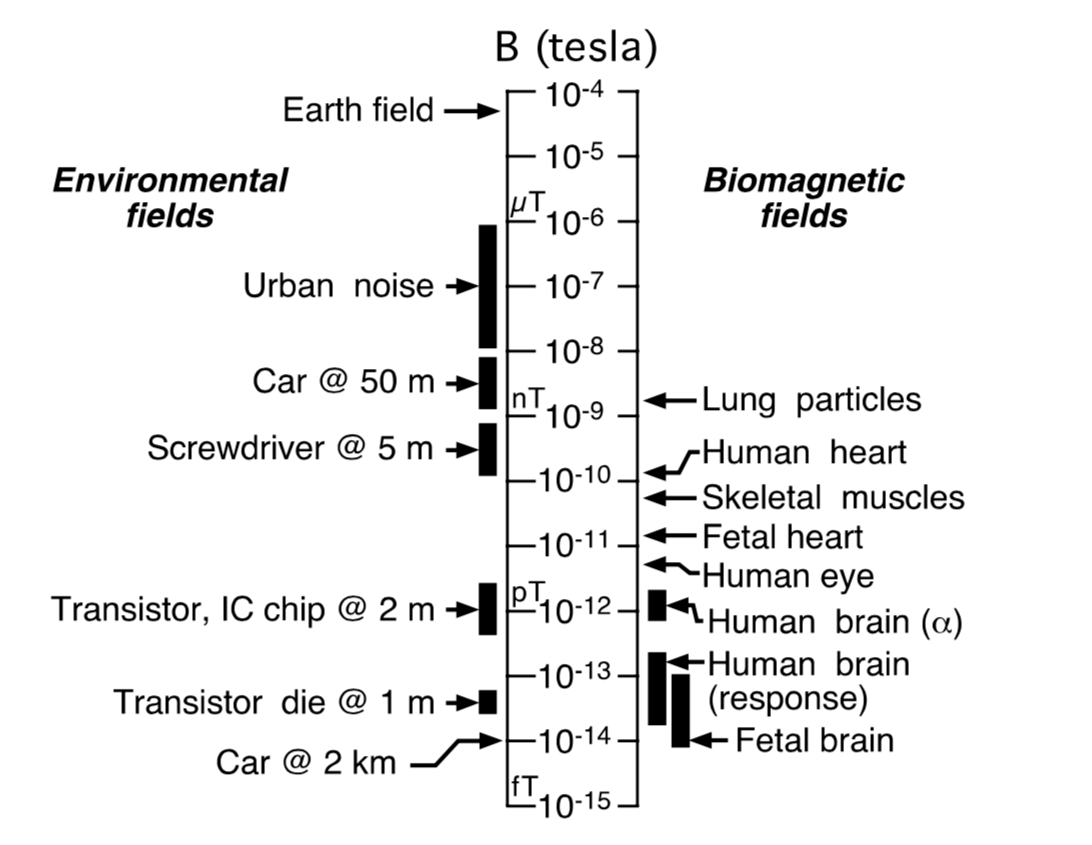
\includegraphics[width=0.7\linewidth]{./images/chapter1/noise_sources.png}\caption{A logarithmic scale showing the magnetic field strength of many sources of interference in MEG data. Figure adapted from \cite{Vrba1999}.}\label{fig_1_n0}
	\end{center}
\end{figure}

\subsection{Magnetically shielded rooms}
A magnetically shielded room (MSR) is the simplest method to reduce the effect of external magnetic noise on MEG data. Typically the MSR consists of alternating layers of aluminium and μ-metals, which have separate functions in shielding the MEG. μ-metals, which are normally an iron-nickel alloy, have a high relative permeability ($\mu_r \simeq 100,000$; \citealt{Hamalainen1993}). The result is that magnetic fields which permeate the shielding will prefer to travel the path of greatest permeability, namely around the walls of the MSR and away from the SQUIDs. The aluminium layers are included to shield the MEG from eddy currents from AC sources and RF interference. MSRs are particularly effective in shielding high frequency field changes; with attenuation of 100 Hz magnetic fields of 50-60 dB. However the effectiveness is less pronounced at lower frequencies, with infra-slow (<0.1 Hz) being attenuated by around 20 dB.

\subsection{Hardwired gradiometers}
Whilst the magnetically shielded room provides a high level of signal attenuation, it is still insufficient for making measurements with a simple SQUID magnetometer as the magnitude of the noise is still orders of magnitude larger than that of the neuromagnetic signals. Another solution (which is employed in the CTF scanner in Nottingham) is the modification of the flux transformer to measure the magnetic field gradient instead of the magnetic field. It is known that the magnetic field strength of a current dipole follows the inverse square law. So it follows that, near a source the field gradient is large, whereas for a source further away the gradient is much lower. With this in mind we can modify the pickup coil of the magnetometer to effectively measure the field gradient. Figure \ref{fig_1_n1}A shows the basic geometry of the pickup coil in a magnetometer, which is a loop of wire that is wound in one direction. The gradiometer on the other hand has a second loop a baseline distance, $b$, from the original, which is wound in the opposite direction. When a time varying magnetic field passes through the coils, it induces currents which are oppositely directed, so a component of that field will cancel out. Figure \ref{fig_1_n1}B shows how this reduces external interference. For a nearby source, as the difference in field magnitude between the two coils should be large, very little is cancelled out. However for far away sources, the fields should be approximately similar and so they are almost entirely nullified. Gradiometers come in two varieties, axial gradiometers, which stack their coils radially from the head surface, and planar gradiometers, which have their coils shifted tangentially and so measure gradients in a perpendicular orientation. Gradiometers allow for the effective noise reduction in recorded MEG signals, but this does come at the expense of reduced sensitivity to deeper sources in the brain. It should be noted that the choice of baseline distance between two coils needs to be optimised, due to the fact that the amplitude of the true neuronal signal detected is attentuated. Should the baseline be too short, the improvement in SNR will not be sufficient; too long and the overall reduction in signal amplitude will too reduce. The optimal baseline for gradiometers placed near the head is typically between 3-8 cm \cite{Vrba2001}. 

\begin{figure}[b!]
	\begin{center}
		\includegraphics[width=\linewidth]{./images/chapter1/figure_n1.png}\caption{Introduction to gradiometry. A) The configuration of MEG pickup coils. The arrows indicate the direction of the coil winding. B) The effect of 1st order gradiometer on inteference. As only the difference between field measurements at $r_1$ and $r_2$ is kept, the effect of the stronger but distal noise source is greatly diminished.}\label{fig_1_n1}
	\end{center}
\end{figure}

\clearpage
\subsection{Synthetic gradiometers}
The gradiometers in Figure \ref{fig_1_n1}A are the family of first order gradiometers. Their noise cancellation properties in conjunction with the passive shielding of the MSR, are good but still can be improved by incorporating higher order field gradients into the measurements. It is possible to build higher order gradiometers for better noise cancellation \citep{Vrba1982}, but in practice they are bulky and impractical for use in MEG. However there is an elegant alternative, using a combination of reference gradiometers distal to the head, we are able to form a synthetic higher order gradiometer \citep{Vrba1991}. In order to illustrate how an n\textsuperscript{th} order synthetic gradiometer system is formulated we need to first consider a simpler setup; a first order gradiometer synthesized from a magnetometer sensor at a position \textbf{r} and a vector reference magnetometer sensor (which consists of three orthogonal coils) at position \textbf{r}'. A diagram of this arrangement can be seen in Figure \ref{fig_1_n2}A.

\begin{figure}[b!]
	\begin{center}
		\includegraphics[width=\linewidth]{./images/chapter1/figure_n2.pdf}\caption{An illustration of gradiometer synthesis. A) Synthesis of a first order gradiometer from a magnetometer sensor near the head and a vector magnetometer reference. B) Synthesis of a second order gradiometer from two hardware first order gradiometers.}\label{fig_1_n2}
	\end{center}
\end{figure}

The magnetometer sensor measures the magnetic field perpendicular to the plane of the coil. If the coil's normal vector is \textbf{P}, the gain of the sensor is $\alpha_P$ and the external field at the vicinity of the coil is \textbf{B}(\textbf{r}), then the measured field would be given by

\begin{equation}
m_P(\mathbf{r})=\alpha_P\big(\mathbf{P\cdot B}(\mathbf{r})\big).
\end{equation} If the vector magnetometer coils each have the same gain $\alpha_R$ as each other, then the output will be given by 

\begin{equation}
R_k(\mathbf{r}')=\alpha_RB_k(\mathbf{r}'),
\end{equation} where $k=1,2,3$. $B_k(\mathbf{r}')$ are the three orthogonal components of the magnetic field measured at position \textbf{r}' and the three components of $R_k(\mathbf{r}')$ can be concatenated  to form the magnetometer output vector \textbf{R}(\textbf{r}'). The first order gradiometer output is given by:

\begin{equation}
g^{(1)}=m_P(\mathbf{r})-\frac{\alpha_P}{\alpha_R}\big(\mathbf{P} \cdot\mathbf{R}(\mathbf{r}')\big). \label{eqn_1_19}
\end{equation} Expansion of the magnetic field using the first two terms of a Taylor series about the origin gives:

\begin{equation}
\mathbf{B}(\mathbf{r}') = \mathbf{B}(\mathbf{r})+\sum_{k=1}^{3}\frac{\partial \mathbf{B}}{\partial x_k}(x_k'-x_k), 
\end{equation} where $x_k$ represents the three orthogonal components of \textbf{r} and likewise, $x_k'$ represents the three orthogonal components of \textbf{r}'. This can be rewritten in terms of the first gradient tensor, thus:
\begin{equation}
\begin{bmatrix}
B_{x_1'} \\ B_{x_2'} \\ B_{x_3'}
\end{bmatrix} 
= \begin{bmatrix}
B_{x_1} \\ B_{x_2} \\ B_{x_3}
\end{bmatrix}
+ \begin{bmatrix}
\frac{\partial \mathbf{B}_{x_1}}{\partial x_1} & \frac{\partial \mathbf{B}_{x_1}}{\partial x_2} & \frac{\partial \mathbf{B}_{x_1}}{\partial x_3} \\
\frac{\partial \mathbf{B}_{x_2}}{\partial x_1} & \frac{\partial \mathbf{B}_{x_2}}{\partial x_2} & \frac{\partial \mathbf{B}_{x_2}}{\partial x_3} \\
\frac{\partial \mathbf{B}_{x_3}}{\partial x_1} & \frac{\partial \mathbf{B}_{x_3}}{\partial x_2} & \frac{\partial \mathbf{B}_{x_3}}{\partial x_3} 
\end{bmatrix}
\begin{bmatrix}
x_1' - x_1 \\ x_2' - x_2 \\ x_3' - x_3
\end{bmatrix} \label{eqn_1_20}
\end{equation} Defining a baseline $\mathbf{b} = \mathbf{r}-\mathbf{r}'$ and $\Delta\mathbf{B} = \mathbf{B}(\mathbf{r}')-\mathbf{B}(\mathbf{r})$, Equation \ref{eqn_1_20} can be rearranged and collapsed down to

\begin{equation}
\Delta \mathbf{B} = \mathbf{G}^{(1)}\mathbf{b},
\end{equation} where $\mathbf{G}^{(1)}$ is the first order gradient tensor. With this we can re-express Equation \ref{eqn_1_19} as

\begin{equation}
g^{(1)} = \alpha_P\mathbf{P}\mathbf{G}^{(1)}\mathbf{b}. \label{eqn_1_22}
\end{equation} What Equation \ref{eqn_1_22} shows is that a synthetic first order gradiometer output is proportional to a projection of the first gradient tensor to the primary orientation of a coil \textbf{P} and the baseline, \textbf{b}. This principle of gradiometer synthesis can be expanded to higher orders. Figure \ref{fig_1_n2}B shows the formulation of a second order gradiometer using two first order gradiometers. The first order baselines (displacement between magnetometer coils) are labelled $\mathbf{b}_1$ and $\mathbf{b}_1'$ and the second order baseline (displacement between individual gradiometer centres), labelled $\mathbf{b}_2=\mathbf{r}-\mathbf{r}'$. The Taylor expansion of the the gradient to a second order around a generalised coordinate \textbf{r} is $\mathbf{G}(\mathbf{r})=\mathbf{G}^{(1)}+\mathbf{G}^{(2)}\mathbf{r}$, so the first order gradiometer for the two gradiometers can be written as 

\begin{equation}
\begin{aligned}
g &= \alpha_G\mathbf{P}\big(\mathbf{G}^{(1)}+\mathbf{G}^{(2)}\mathbf{r}\big)\mathbf{b}_1\\
g' &=  \alpha_{G'}\mathbf{P}'\big(\mathbf{G}^{(1)}+\mathbf{G}^{(2)}\mathbf{r}'\big)\mathbf{b}_1'
\end{aligned}
\end{equation} If we assume that $\mathbf{p}\parallel\mathbf{p}'$ and $\mathbf{b}_1\parallel\mathbf{b}_1'$ we can use similar steps to those used to derive the first order gradient to express the second order output

\begin{equation}
\begin{aligned}
g^{(2)}&=g-\frac{\alpha_G}{\alpha_{G'}}\frac{b_1}{b_1'}g' \\
&\approx \alpha_G\mathbf{PG}^{(2)}\mathbf{b}_2\mathbf{b}_1,
\end{aligned}
\end{equation} this procedure can be generalised to the n\textsuperscript{th} order and shows that high order gradiometers can be synthesized from a combination of magnetometers and gradiometers. The CTF MEG system in Nottingham can synthesize third order gradiometers with its sensors, and the third order gradient output is given as

\begin{equation}
g^{(3)} \approx \alpha_G\mathbf{PG}^{(3)}\textbf{b}_3\textbf{b}_2\textbf{b}_1
\end{equation} where $\mathbf{b}_3$ is the third order baseline.

\subsection{Software approaches}
Not all MEG laboratories use the hardware approaches mentioned, this may be down to a personal choice or due to a lack of availability (for example MEG systems manufactured by Elekta do not come with a reference array to allow for synthetic gradiometry). Instead, there are noise reduction approaches which exist in the software domain which can remove environmental contaminants, however this comes at the detriment of making the data rank deficient (i.e. the rank of the data is less than the number of sensor timecourses\footnote{Technically this also applies to using a reference array to regress out interference. However in that case if you have 300 sensors, of which 25 are references sensors, you ensure that the rank of the data post reference correction is 275 and analyse the non-reference channels. For software correction you don't have the luxury of redundant channels and so the analysed data is rank deficient.}); here we describe two such methods. 

\subsubsection{MaxFilter\textsuperscript{TM}}
For Elekta systems, there is a suite of software to accommodate for the lack of reference array which come under the name of MaxFilter\textsuperscript{TM}. At the core of it is an algorithm known as Signal Space Separation (SSS; \citealp{Taulu2004}). SSS assumes that the sensors are far enough away from all magnetic field sources that they are oversampling their field patterns. From this they derive a vector basis set which best describes the measurements and satisfy the equation $\mathbf{\nabla}^2A=0$, where \textit{A} is the magnetic scalar potential. This results in a set of spherical harmonic terms, with certain terms associated with sources within the head and others which are external interference. The external components are regressed out of the data. 

\subsubsection{ICA Denoising}
A popular approach to clean data post-hoc is the use of temporal independent component analysis (tICA) to identify sources of interference \citep{Mantini2007}. tICA is a blind source separation which assumes data from multiple simultaneous recordings contain mixed sources which can be separated. The mathematics for tICA are covered in Section \ref{sec_bf_v_mn}, but in short, tICA separates sources and provides coefficients which correspond to a weighted sum of the recordings which make up that source. If these sources are sorted in order of kurtosis, you find that sources of biological noise (magnetomyogram, magnetoculargrams and magnetomyograms) tend to be the first components due to their non-gaussianity, and AC mains interference is the final component. These components are then, like with SSS, regressed out of the recordings.  

\clearpage
\section{Experimental procedure for data collection}\label{sec_data_acq}
In MEG experiments, there are many steps which are required to ensure that the data acquired are of an acceptable standard and the subject is safe at all times. Below are a set of operating procedures which were adhered to for all of the experimental investigations in this thesis. 

Prior to data acquisition, a subject is provided with an information sheet about the investigation, a safety screening test and a consent form for them to fill in. Should a participant be happy to consent to the experiment, pass safety screening and remove all metal from their person, they can proceed to be scanned. 
 
Figure \ref{fig_1_a1} shows a simplified experimental setup of the MEG acquisition suite. Inside the magnetically shielded room, the subject is positioned supine and space between their head and the dome of the MEG are filled with padding to minimise head movement during the experiment. Attached to a participant are three head position indicator coils, which are placed on the nasion, and left/right preauricular regions. These coils are energised periodically during data acquisition in order to localise the subject's head in the scanner and to track their head movement. During the experiment, measurements from the SQUIDs are handled and digitised by an electronics rack and sent to an acquisition which records the data to disk. A stimulus computer is used to provide audio/visual/computer stimuli in conjuction with a series of peripherals such as projectors, air powered earphones and optical keypads. The acquisition and stimulus computers are linked so that markers, which indicate when key stimuli occur are automatically embedded into a dataset. Unless explicitly stated, all data within this thesis were recorded at a sampling rate of 600 Hz with the third order synthetic gradiometers utilised. 

As the MEG system contains a dewar of liquid helium to keep the SQUIDs at superconducting temperature, safety precautions must be taken to control for the unlikely case of a dewar breach. Risks to the subject range from burns from the extreme low temperatures to death from asphyxiation. Should the subject notice something unusual, a two way intercom allows the subject to notify the MEG operator (likewise it allows the operator to communicate with the subject useful information). There is also a video camera to allow visual assessment within  the MSR and finally there are a series of sensors which measure O\textsubscript{2} levels in the MSR and helium evaporation rate within the dewar. Should levels cross an unacceptable threshold alarms will sound, notifying the operator to evactuate the subject from the MSR. 

Post acquisition, the data undergoes quality control. If the subject has moved their head more than 5 mm during the course of the experiment, the data are discarded (until such a time that we can retroactively correct for head motion in a CTF scanner). After this, each trial is inspected (if the data are from a resting state experiment, it is typically cut into 10 s epochs) for artefacts associated with eye-blinks or the eletromyogram or SQUID resets (Figure \ref{fig_1_a2}). Should excessive interferences from these sources be present the trial is discarded. Finally the data are DC offset corrected to remove infra-slow drift. 

\begin{figure}[h!]
	\begin{center}
		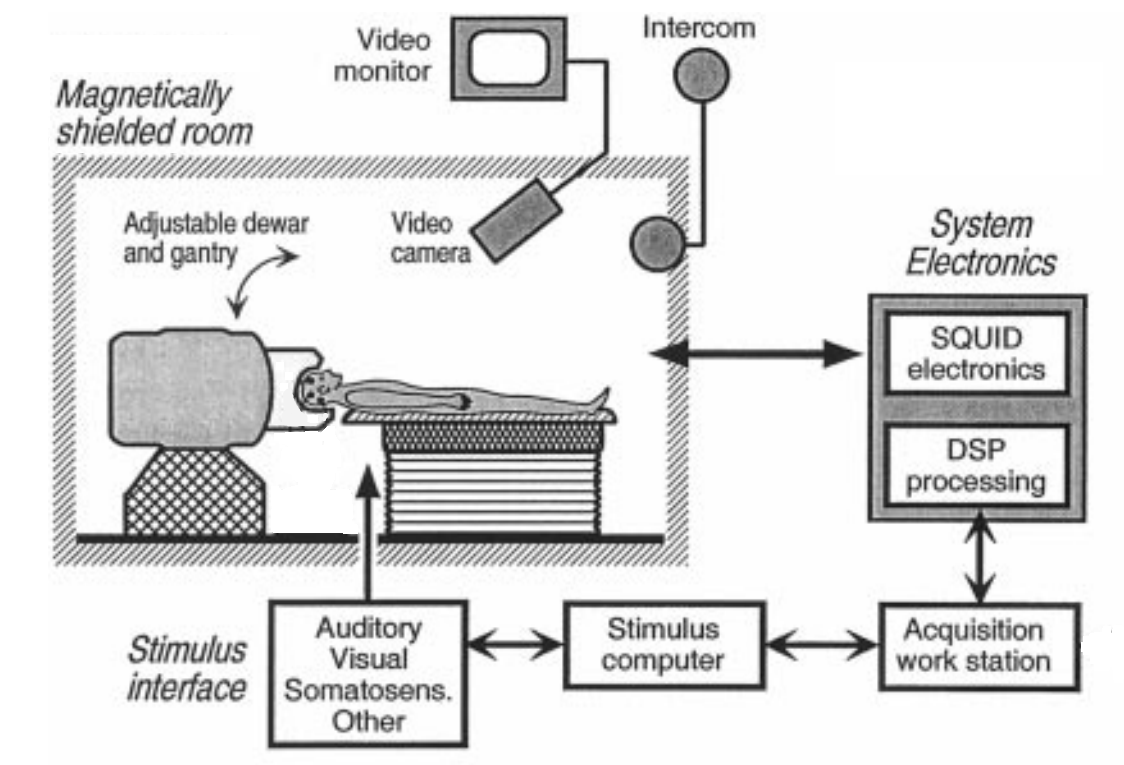
\includegraphics[width=\linewidth]{./images/chapter1/experimental_setup.png}\caption{A simplified diagram of the experimental setup of the MEG suite. Figure adapted from \cite{Vrba2001}.}\label{fig_1_a1}
	\end{center}
\end{figure}
\clearpage

\begin{figure}[h!]
	\begin{center}
		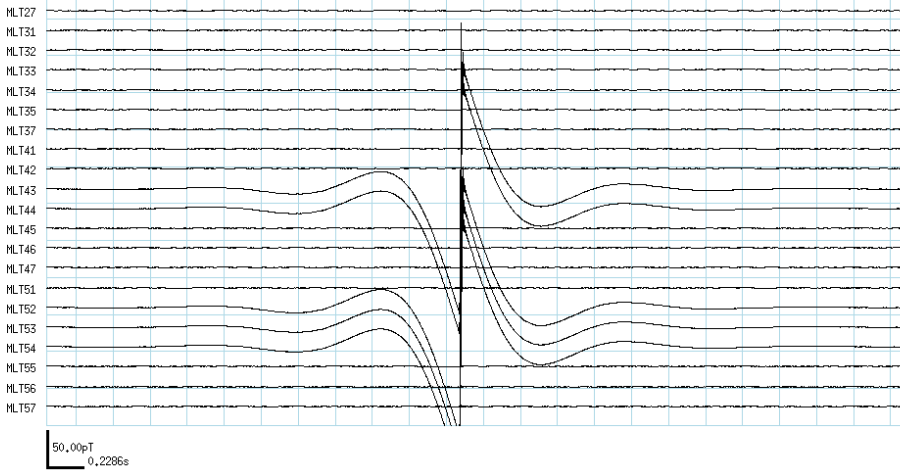
\includegraphics[width=0.78\linewidth]{./images/chapter1/SQUID_RESET.png}\caption{Example of a SQUID reset artefact. Note that the associated field with the reset is approximately 0.5 nT and so dwarfs any neuromagnetic signals.}\label{fig_1_a2}
	\end{center}
\end{figure}

\subsection{Data coregistration}
For reasons which are discussed in detail in Chapter \ref{chapter_meg_source}, we want to be able to reconstruct data in source space. Whilst not strictly necessary for source reconstruction in the MEG, knowing exactly where the brain was inside the MEG dome allows us to superimpose source reconstructed data onto an anatomical image of the brain to aid functional analysis. However as our MEG system can only image brain function, we need to coregister the MEG data to a separately acquired MRI of the participant if we want to be able to perform source analysis later. The head position indicators, which track head motion within the MEG are used as fiducial markers for coregistering across the imaging modalities. The participant's head surface is digitised along with the relative positions of the fiducial coils using a Polhemus FASTRAK 3D digitiser system. The digitiser uses three concentric low frequency transmitters placed behind the subject and a receiver placed on the vertex of the subjects head to triangulate the position of a stylus, which is used to draw the shape of the scalp and face of the participant (Figure \ref{fig_1_a3}A). This creates a 3D representation of the subject's head (shown as the blue dots in Figure \ref{fig_1_a2}B). Anatomical MR images are acquired using either a 3 T or 7 T Philips Acheiva MRI scanner. A T\textsubscript{1}-weighted MR image is acquired using an MPRAGE sequence \citep{BrantZawadzki1992} at 1 mm\textsuperscript{3} isotropic resolution. A 3D head surface from the anatomical is extracted using edge detection methods and the digital head surface is matched using an iterative closest point algorithm \citep{Besl1992}. The result of the coregistration is shown in Figure \ref{fig_1_a3}C, where the purple point represents the derived location of the nasion head position indicator during this experiment. 

\begin{figure}[h!]
	\begin{center}
		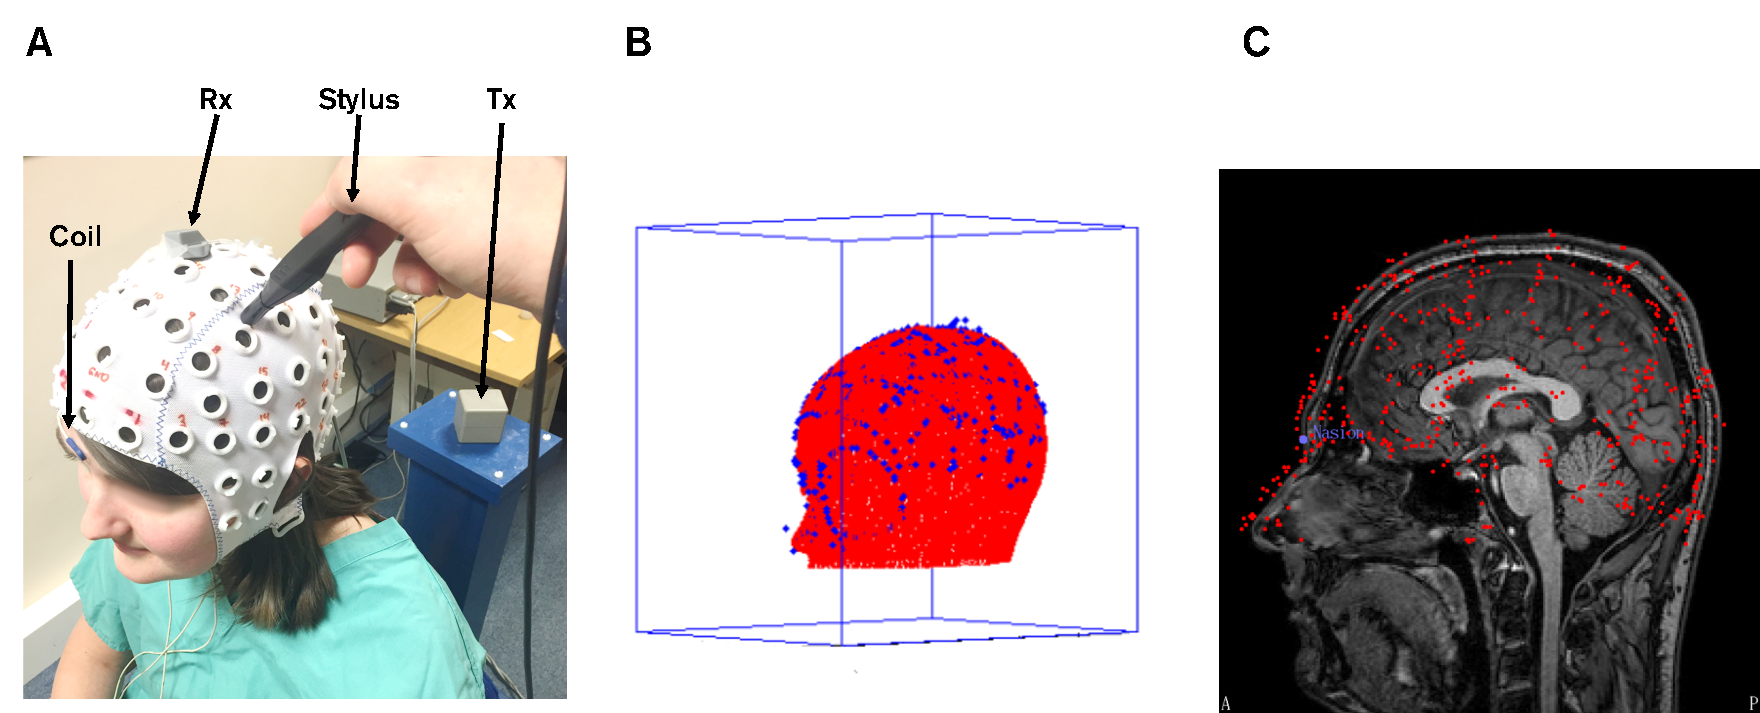
\includegraphics[width=\linewidth]{./images/chapter1/coreg.png}\caption{Data coregistration procedure. A) Digitisation of the head surface using the Polhemus ISOTRAK. B) The digitised head surface (blue dots) are aligned to a head surface derived from an MRI of the participant. C) The result of coregistration, the green dot represents the derived location of the nasion head position indicator. }\label{fig_1_a3}
	\end{center}
\end{figure}

\section*{Summary}

In this chapter a brief overview on the origins on the MEG signal has been given, and the theoretical and practical aspects of data acquisition in a MEG experiment were explained. We have seen that it is possible to measure the extracranial magnetic field associated with dendritic current flow using SQUIDs and that even though they are several orders of magnitude weaker than other sources of interference, it is possible to remove many of these noise sources to be left with data which is a better representative of what is truly inside the sensor dome of the MEG. In the next chapter we move on to discuss how we can reconstruct the sensor data from MEG to derive 3D images of brain current.